\documentclass[conference]{IEEEtran}
\IEEEoverridecommandlockouts
% The preceding line is only needed to identify funding in the first footnote. If that is unneeded, please comment it out.
\usepackage{cite}
\usepackage{amsmath,amssymb,amsfonts}
\usepackage{algorithmic}
\usepackage{graphicx}
\usepackage{textcomp}
\usepackage{xcolor}
\usepackage{tabularx}
\def\BibTeX{{\rm B\kern-.05em{\sc i\kern-.025em b}\kern-.08em
    T\kern-.1667em\lower.7ex\hbox{E}\kern-.125emX}}
\begin{document}

\title{Modeling and Robust Control of Ball Plate System using different control methodologies\\
}

\author{\IEEEauthorblockN{1\textsuperscript{st} Given Name Surname}
\IEEEauthorblockA{\textit{dept. name of organization (of Aff.)} \\
\textit{name of organization (of Aff.)}\\
City, Country \\
email address or ORCID}
\and
\IEEEauthorblockN{2\textsuperscript{nd} Given Name Surname}
\IEEEauthorblockA{\textit{dept. name of organization (of Aff.)} \\
\textit{name of organization (of Aff.)}\\
City, Country \\
email address or ORCID}
}
\maketitle

\begin{abstract}
Different control mechanisms for balancing the ball plate system (BPS)  have been discussed in this paper. The ball plate system is a popular nonlinear control problem and various control system strategies have been put forward to approach the problem. We put forward the analysis and comparison of three such different control approaches namely: Sliding Mode Control (SMC), Proportional Integral Derivative (PID), and Linear Quadratic Regulator (LQR). The comparison between the strategies is based on the performance of trajectory and fixed point tracking, and how the system reacts to noise and external disturbance in each case.
\end{abstract}

\begin{IEEEkeywords}
component, formatting, style, styling, insert
\end{IEEEkeywords}

\section{Introduction}
The ball plate system is a very popular educational model to teach and validate various control strategies. The control objective of the ball and plate problem is to balance a ball or to make it track the desired trajectory, on a flat plate, solely by tilting the plate relative to the horizontal plane. This system is of particular interest to the control community because it allows the user to study and validate a wide class of both linear and nonlinear control schemes, before applying them to real-life applications that exhibit similar dynamics. The ball moves on a plate fixed with motors that control the inclination of the plate based on the control input obtained and the ball has 2DOF of motion (along the X and Y-axis). The control algorithm is first verified using the derived nonlinear simulation model in MATLAB for different methods.

The ball and plate system is an extension of the Ball and Beam system \cite{b1}. It is considered a benchmark model of a driftless nonholonomic system. A state feedback controller using the pole assignment method was designed in \cite{b2} to maintain a desired position of the sphere over the plane. A computer vision technique allowed us to measure the two-dimensional position of the sphere over the plane in real-time. \cite{b3} considered the feedback delay in the control loop for determining the state-space model of the Ball-Plate System, and secondly, based on the geometric method and the state feedback control an observer is synthesized. The ball and plate system is used as a nonlinear, uncertain, and MIMO system to verify the effectiveness of the proposed controller.  The invasive weed optimization (IWO) method, which is one of the metaheuristic optimization algorithms, is used to obtain the optimal parameters of the proposed controller \cite{b4}. In \cite{b5} the authors discuss the use of PD position controller and PD angle controller to control the ball and plate system. Design and Implementation of a Ball-Plate Control System using computer vision as a feedback sensorand Python Script for Educational Purposes in STEM Technologies is proposed in \cite{b6}. In their paper, Mujadin et al. \cite{b7} developed the ball plate system control using a resistive touch screen as the sensor position of the ball.  Cheng et al. \cite{b8} present a skillful robotic wrist system using a visual servo control technique to demonstrate the dexterity of the mechanical wrist from the viewpoint of table tennis whereas the ball and plate system is chosen as the basic stage of this work. Dusek et al. \cite{b9} present the modeling of the ball and plate systems based on first principles which consider the balance of torques and forces.  Ibrahim Mustafa Mehedi et al. \cite{b10} presented fractional order controller design for the beam and ball system. \cite{b11} discusses an efficient method to improve the balancing and tracking of the trajectory of the BOPS based on machine learning (ML) algorithm with the Pseudo proportional-derivative (PPD) controller. 
Various control methods are used to maintain the position of ball on plate such as, Fuzzy control \cite{b12}, PID\cite{b13}, the Sliding Mode Control (SMC)\cite{b14}, LQR\cite{b15}. We present the analysis and comparison of three such methods: PID, LQR and SMC.

The  BPS is marginally stable since it contains a double pole in the origin. This results in the system having only non-decaying oscillatory components in its step response when introduced to a feedback loop. To gain stability and enhance the performance of the system a PID controller is introduced. Values of Kp, Ki, and Kd determine the control output that is required to attain a stable system response. Values of Kp, Ki and Kd are established through an iterative process in MATLAB.The Linear Quadratic Regulator (LQR) is a well-known method that provides optimally controlled feedback gains to enable the closed-loop stable and high-performance design of systems. Sliding mode control is a robust control strategy that guarantees a suitable response even in the face of model imprecisions and external disturbances. Robustness is achieved by employing a discontinuous control action.

Control theory and its applications are crucial when operating within the area of dynamic systems. The system should be able to recover and compensate for disturbances and external actions imposed on a given system being inherently unstable or semi-stable. Based on the simulation, a comparison of the given three strategies is also made based on their response to external disturbances. 



\section{Modeling}

\subsection{System Description}

The ball-plate system developed and modeled in this case is a 2DoF system, having a simple plate and a ball placed over it. The inclination in both dimensions is provided by two motors, mounted in perpendicular directions such that the inclination provided by one motor doesn’t effect the motion in other direction. The inclination of the plate in both the directions can be utilized to balance the ball at the desired position on the plate, as well as make the ball follow a trajectory on it.
\begin{figure}[htbp]
\centerline{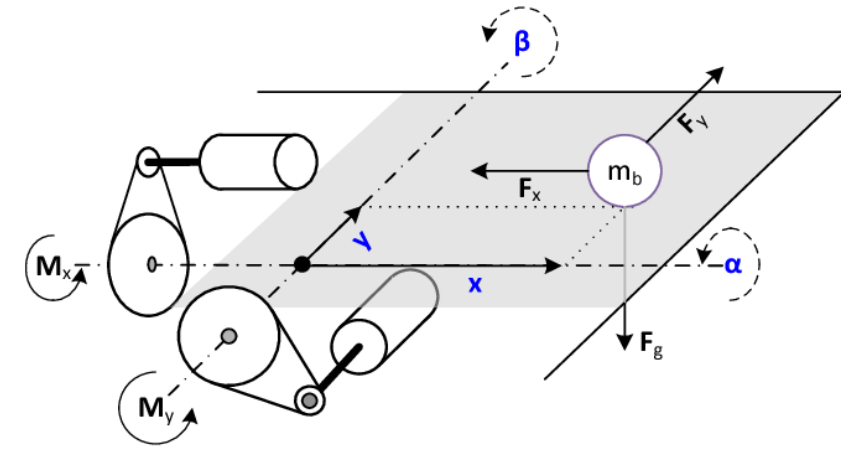
\includegraphics[width=0.5\textwidth]{FBD.png}}
\caption{Free Body Diagram of System.}
\label{fig1}
\end{figure}

\subsection{System Equations}
The dynamic equations of the system are derived in this section. Certain assumptions are made regarding the system which simplify the model: (1) There is no slipping of ball on the plate (2) Friction everywhere else is neglected (3) The ball is homogenous and symmetrical (4) The ball and the plate are in contact all the time. Lagrangian method is used to derive these equations. The Euler-Lagrange equation for the ball and plate system is: 

\begin{equation}
\frac{d}{dt}\left(\frac{\partial L}{\partial q_{i}}\right) - \frac{\partial L}{\partial q_{i}} = Q_{i}\label{eq1}
\end{equation}

Where $q_{i}$ represents the i direction coordinate and $Q_{i}$ stands for the composite force in the i direction. $L$ is defined as the Lagrangian of the system.
\\The system can be described as having 4 degrees of freedom. Two, of the ball in the x and y directions, and two of the plate inclination, with rotational axis of the plate in both of these directions. Table \ref{table1} describes the variables of the system:

\begin{table}[h!]
\caption{System Variables and Constants}
\begin{center}
%\begin{tabularx}{0.4\textwidth} { 
%  | >{\centering\arraybackslash}X 
%  | >{\centering\arraybackslash}X | }
\begin{tabular}{| c | c |}
 \hline
 Variable & Description \\
\hline
x$_{b}$  & x coordinate of ball on plate \\
\hline
y$_{b}$  & y coordinate of ball on plate  \\
\hline
$\dot x_{b}$  & translational velocity of ball along x-axis  \\
\hline
$\dot y_{b}$  & translational velocity of ball along y-axis  \\
\hline
$\alpha$ & angle of inclinatin of plate along x-axis  \\
\hline
 $\beta$  &  angle of inclinatin of plate along y-axis\\
\hline
$\dot \alpha$ & angular speed of plate along x-axis  \\
\hline
 $\dot \beta$ & angular speed of plate along y-axis  \\
\hline
m$_{b}$  & mass of ball \\
\hline
 I$_{b}$  & Moment of Inertia of ball  \\
\hline
 I$_{b}$  & Moment of Inertia of plate  \\
\hline
 M  & Mass of plate \\
\hline
 w$_{x}$  & angular speed of ball along x-axis  \\
\hline
 w$_{y}$  & angular speed of ball along y-axis  \\
\hline
 T$_{x}$ & Torque applied on the plate along x-axis  \\
\hline
 T$_{y}$  & Torque applied on the plate along y-axis \\
\hline
 r$_{b}$ & radius of ball \\
\hline
\end{tabular}\label{table1}
\end{center}
\end{table}

The inclination is with respect to the horizontal plane and the coordinates are according to the position of the ball on the plate with respect to the centre of the plate.
Then, the kinetic energy of the system ($T$) can be defined as the sum of kinetic energies of the ball and the plate: 
\begin{equation}
T = T_{b} + T_{p}\label{eq2}
\end{equation}
The kinetic energy of the ball is the sum of both translational and rotational energies with respect to its centre of mass:
\begin{equation}
T_{b} = \frac{1}{2} m_{b} \left( \dot x_{b}^{2} + \dot y_{b}^{2} \right) +  \frac{1}{2} I_{b} \left(w_{x}^{2} + w_{y}^{2} \right)\label{eq3}
\end{equation}
Here, we can replace the values of $w_{x} \mbox{ and } w_{y}$ as $ \dot x_{b} \! = \! w_{x}r_{b} \mbox{ and } \dot y_{b} \! = \! w_{y}r_{b}$.
The kinetic energy of the plate is the rotational energy of a square plate with a point mass (ball assumed as a point mass) attached at coordinates $(xb, yb)$ with respect to its centre of mass:
\begin{equation}
T_{p} = \frac{1}{2} \left(I_{b} + I_{p}\right) (\dot \alpha^{2} + \dot \beta^{2} ) + \frac{1}{2} m_{b} ( x_{b} \dot \alpha + y_{b}\dot \alpha )^{2}\label{eq4}
\end{equation}
The relative potential energy of the system is considered as the relative potential energy of the ball with respect to its position at origin at zero inclination, and the change in potential energy of the plate is neglected:
\begin{equation}
V = V_{b} = m_{b} g h = m_{b} g \left( x_{b}sin\alpha + y_{b}sin\beta\right)\label{eq5}
\end{equation}
Thus, Lagrangian of the system is:
\begin{equation}
L = T - V = T_{b} + T_{p} - V_{b}\label{eq6}
\end{equation}
Using equations \ref{eq1}-\ref{eq5} we derive the dynamical equations of the system: 
%\begin{align}
\begin{equation}
\frac{\partial L}{\partial \dot x_{b}} =  \left( m_{b} + \frac{I_{b}}{r_{b}^{2}} \right) (\dot x_{b})
\label{eq7}\end{equation}
\begin{equation}
\frac{\partial L}{\partial x_{b}} = m_{b}(x_{b}\dot\alpha^{2} + y_{b}\dot\alpha\dot\beta) - m_{b}gsin\alpha
\label{eq8}\end{equation}
\begin{equation}
\frac{\partial L}{\partial \dot \alpha} = (I_{b} + I_{p})\dot\alpha + m_{b}(x_{b}^{2}\dot\alpha + x_{b}y_{b}\dot\beta)
\label{eq9}\end{equation}
\begin{equation}
\frac{\partial L}{\partial \alpha} = -m_{b}gx_{b}cos\alpha
\label{eq10}\end{equation}
\begin{equation}
\begin{split}
\frac{d}{dt}\left(\frac{\partial L}{\partial \dot x_{b}}\right) - \frac{\partial L}{\partial x_{b}} = \left(m_{b} + \frac{I_{b}}{r_{b}^{2}}\right)\ddot x_{b} \\- m_{b}(x_{b}\dot\alpha^{2} + y_{b}\dot\alpha\dot\beta) + m_{b}gsin\alpha = 0
\end{split}
\label{eq11}\end{equation}
\begin{equation}
\begin{split}
\frac{d}{dt}\left(\frac{\partial L}{\partial \dot \alpha}\right) - \frac{\partial L}{\partial \alpha} = (I_{b} + I_{p}  + m_{b}x_{b}^{2})\ddot \alpha + \\2m_{b}x_{b}\dot x_{b} \dot \alpha + m_{b}x_{b} y_{b} \ddot \beta + m_{b}y_{b}\dot x_{b} \dot \beta \\+ m_{b}x_{b}\dot y_{b} \dot \beta + m_{b}gx_{b}cos\alpha = T_{x}
\end{split}
\label{eq12}\end{equation}
%\end{align}

Similarly, equations can be obtained for y-direction. \\
These equations can be manipulated to represent the system in vector form. Henceforth, the way in which these vectors are written determine the way the system is modeled and controlled.

\subsection*{Approach 1}
The system inputs are taken as plate angles rather than the torques on the plate. In a way, this approach limits the system to just the segment of interest i.e., the position of the ball. The state vector and dynamic equation of the system are:
\begin{equation} X = \begin{bmatrix}
x \\ \dot x \\ y \\ \dot y
\end{bmatrix} = 
\begin{bmatrix}
x_{1} \\ x_{2} \\ x_{3} \\ x_{4}
\end{bmatrix} \>\>;\>\>
\dot X = \begin{bmatrix}
\dot x \\ \frac{x_{b} \dot \alpha^{2} + y_{b} \dot \alpha \dot \beta - gsin\alpha}{C_{1}} \\ \dot y \\ \frac{y_{b} \dot \beta^{2} + x_{b} \dot \alpha \dot \beta - gsin\beta}{C_{1}}
\end{bmatrix}\label{eq13}
\end{equation} 
Where, $C_{1} = 1+\frac{I_{b}}{m_{b} r_{b}^{2}}$\\
It is evident from these equations that the non-linearity in this system is too complex to be worked upon. Thus the system is linearized and the equations are decoupled in x and y directions to apply individual control laws in independent directions x and y. Such approach is relevant when the control input is directly the angle of the plate, and hence the hardware implementation of the system involves servo motors whose angles directly map on to the angle of inclination of the plates.

\subsection*{Approach 2 }
In this approach, the entire system, including the plate is modeled. Thus the state vector and the dynamic equation of the system are: 
\begin{equation}
X = \begin{bmatrix}
x \\ \dot x \\ \alpha \\ \dot \alpha \\ y \\ \dot y \\ \beta \\ \dot \beta
\end{bmatrix}
%\begin{bmatrix}
%x_{1} \\ x_{2} \\ x_{3} \\ x_{4} \\ x_{5} \\ x_{6} \\ x_{7} \\ x_{8}
%\end{bmatrix}
;
\dot X = 
\begin{bmatrix}
\dot x 
\\ \frac{x_{b} \dot \alpha^{2} + y_{b} \dot \alpha \dot \beta - gsin\alpha}{C_{1}} 
\\ \dot \alpha
\\  ( T_{x} - 2m_{b}x_{b}\dot x_{b} \dot \alpha - m_{b}x_{b} y_{b} \ddot \beta
\\  \frac{- m_{b}y_{b}\dot x_{b} \dot \beta - m_{b}x_{b}\dot y_{b} \dot \beta - m_{b}gx_{b}cos\alpha )}{C_{2} + m_{b}x_{b}^{2}}
\\ \dot y 
\\ \frac{y_{b} \dot \beta^{2} + x_{b} \dot \alpha \dot \beta - gsin\beta}{C_{1}}
\\ \dot \beta
\\ ( T_{y} - 2m_{b}y_{b}\dot y_{b} \dot \beta - m_{b}x_{b} y_{b} \ddot \alpha
\\ \frac{- m_{b}x_{b}\dot y_{b} \dot \alpha - m_{b}y_{b}\dot x_{b} \dot \alpha - m_{b}gy_{b}cos\beta )}{C_{2} + m_{b}y_{b}^{2}}
\end{bmatrix}\label{eq14}
\end{equation}
Where, $C_{2} = I_{b} + I_{p}$
The control inputs are torques on plates applied by the motors. This approach is thus relevant to those hardware implementations in which electrical command given to the motors (as voltage or current) directly generates proportional amount of torque.



\section{Control Methodology}
The control methodologies adopted for both the approaches to model the system are different. While in the first approach, focus is on the position of the ball and the plates are not monitored, the second approach requires monitoring and control of every aspect, namely- the angular velocities as well as angle of inclinations of plate in both directions in addition to the state of the ball.

\subsection{Method 1: Using PID}
PID control has been implemented to control the position of the ball.The system is dynamically represented as shown in [\ref{eq13}]. The first step is to linearize these equations and decouple the system after making certain assumptions. These decoupled equations are: 
\begin{equation} \ddot x_b = -Csin \alpha \>\>\> ; \>\>\>  \ddot y_b = -Csin \beta \label{eq15}\end{equation} where $C = g/C1$.
Thus the system can be represented in state space form as:
\begin{equation}
\dot X = A X + B U\label{eq16}
\end{equation}
$ A = \begin{bmatrix}
0 & 1 & 0 & 0 \\ 0 & 0 & 0 & 0 \\ 0 & 0 & 0 & 1 \\ 0 & 0 & 0 & 0
\end{bmatrix}$ \> ; \>
$ B = \begin{bmatrix}
0 & 0 \\ -C & 0 \\ 0 & 0 \\ 0 & -C
\end{bmatrix}$ \> ; \>
$ U = \begin{bmatrix}
sin \alpha \\ sin \beta
\end{bmatrix}$\\\\
For small values of alpha and beta, the values $sin \alpha \mbox{ and } sin \beta$ can be approximated as $\alpha \mbox{ and } \beta$.

\subsection*{PID Controller Design}
\begin{figure}[htbp]
\centerline{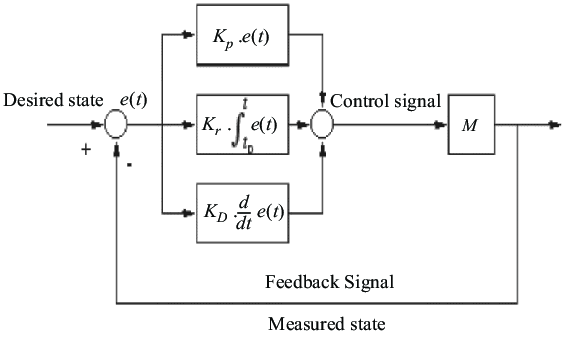
\includegraphics[width=0.4\textwidth]{BDPID.png}}
\caption{Block Diagram of PID Controller}
\label{fig2}
\end{figure}
The desired position of the ball is fed as an input to the system. The error is the difference between the desired position and the current position of the ball, which is minimised through the control input to the system represented by the equation:
\begin{equation}
K_p e(t) + K_i \int_{t_0}^{t} e(t) \,dt + K_d \frac{d}{dt}e(t)
\label{eq17}\end{equation}
Here, the constants $K_p, K_i \mbox{ and } K_d $ are the parameters that need to be tuned to obtain the desired response. Thus with this control law, the overall transfer function of the system can be represented as: 
\begin{equation}
T(s) = C(s)G(s) = (K_p + sK_d + \frac{K_i}{s})(\frac{1}{s^2})
\label{eq18}\end{equation}
From the condition of stability (all poles of this transfer function lie on the left hand side of the complex plane), the following condition has been obtained for the controller: $ K_p K_d > K_i$.
Table \ref{table2} lists all the parameters describing the system.

\begin{table}[h!]
\caption{System parameters for PID controller}
\begin{center}
\begin{tabular}{| c | c | c |}
 \hline
 Parameter & Description & Value\\
\hline
$m_{b}$  & mass of ball  & 4\\
\hline
 $I_{b}$  & Moment of Inertia of ball  & 5\\
\hline
 $I_{p}$  & Moment of Inertia of plate  & 6\\
\hline
 $K_{p}$  & Proportional gain constant  & 7\\
\hline
 $K_{d}$  & Derivative gain constant & 8\\
\hline
 $K_{i}$ & Integral Gain constant & 9\\
\hline
 $e_{t}$  & \multicolumn{2}{c|}{Error between desired and current posiition} \\
\hline
$\frac{d}{dt}e(t)$ &\multicolumn{2}{c|}{Error between desired and current velocities}\\
\hline
$\int_{t_0}^{t} e(t) \,dt$ & \multicolumn{2}{c|}{Error integrated over time}\\
\hline
\end{tabular}\label{table2}
\end{center}
\end{table}


This control law is applied separately in both directions x and y to minimise the individually determined errors in x and y directions respectively. The selection of $K_p, K_i \mbox{ and } K_d $ values give minimum settling time of the system response and negligible steady state error and are selected by hit and trial method.

The above control law is applied to control the position of ball in two scenarios: (i.) Fixed point tracking and (ii.) Trajectory tracking.

(i). Fixed point tracking can further be performed using two approaches, first, giving the final position of the ball and minimising the error between desired position and starting position in minimum time. The second approach is basically trajectory tracking where the desired trajectory is a straight line path from the starting position to the final position and then staying at the final position. This approach finds application in how quickly the ball should reach the final position and taking what path.

(ii). Trajectory tracking makes use of the underlying principles of fixed point tracking where the desired position is constantly changing point by point, and the error between the current position and the desired position at the current moment is minimised, eventually tracing a specific path. A circular trajectory has been traced in this case to show trajectory tracking capability.

\subsection{Method 2 : Using LQR}
Linear Quadratic Regulator is generally employed in applications where a stability problem needs to be addressed. The ball and plate system can also be analysed and presented as a stability problem where the ball needs to be balanced on a fixed position of the plate. The system is dynamically represented in [\ref{eq14}] along with the 8-dimensional state vector. In order to simplify the system dynamics, linearization has been performed about the fixed point selected as origin. A fixed point of the system is a point where the system is stable if untouched. The horizontal position of the plate is stable when the ball is at origin (if the mass of the ball is not considerably less than the mass of the plate). When the ball is displaced from this position, system destabilizes and reaches the minimum energy point (where the vertical position of the ball is lower than its position at origin when the plate is horizontal, so that potential energy falls). In the neighbourhood of this fixed point, the system can be linearized. Hence, for the dynamical equations, Jacobian has been evaluated about the Zero state and following matrices are obtained: 
\begin{equation}\begin{split}
A = \begin{bmatrix}
0 & 1 & 0 & 0 & 0 & 0 & 0 & 0 \\
0 & 0 & -C & 0 & 0 & 0 & 0 & 0 \\
0 & 0 & 0 & 1 & 0 & 0 & 0 & 0 \\
-C_3 & 0 & 0 & 0 & 0 & 0 & 0 & 0 \\
0 & 0 & 0 & 0 & 0 & 1 & 0 & 0 \\
0 & 0 & 0 & 0 & 0 & 0 & -C & 0 \\
0 & 0 & 0 & 0 & 0 & 0 & 0 & 1 \\
0 & 0 & 0 & 0 & -C_3 & 0 & 0 & 0 \\
\end{bmatrix} ; 
B = \begin{bmatrix}
0 & 0 \\
0 & 0 \\
0 & 0 \\
\frac{1}{C_2} & 0 \\
0 & 0 \\
0 & 0 \\
0 & 0 \\
0 & \frac{1}{C_2} \\
\end{bmatrix}
\\\\
\mbox{ and Zero Vector } = X_0 = \begin{bmatrix}0 &0 &0 &0 &0 &0 &0 &0\end{bmatrix}^T
\end{split}\label{eq19}\end{equation}
Where $C_3 = \frac{m_b g}{C_2}$.
The system can now be represented having the state space model:
\begin{align}
\dot X = A X + B U \label{eq20}\\
Y = C X + D U\label{eq21}
\end{align}
where,
\begin{equation}
C = \begin{bmatrix}
1 & 0 & 0 & 0 & 0 & 0 & 0 & 0 \\
0 & 0 & 0 & 0 & 1 & 0 & 0 & 0 \\
\end{bmatrix} ; 
D = \begin{bmatrix}
0 & 0 \\
0 & 0 \\
\end{bmatrix} 
\label{eq22}\end{equation}



\subsection*{LQR Controller Design}
For this linearized state space system, the control input is proportional to the current state and is mathematically written as : <U=-KX> where K is the gain matrix.
The system eventually becomes: <X’ = A-BKX>
The response of this system is determined by the eigenvalues or poles. By controlling matrix K, the poles can be shifted to the left half of the complex plane to stabilize the system. Further, the position of these poles determine the response of the system, in terms of steady state error and settling time.
One method to determine K is using manual pole placement. But it requires the intuition that a chosen eigenvalue will affect the system in the desired way. As its hard to establish a direct relation between the position of various poles and the effect it has on the system, a much more intuitive method has been adopted. Using LQR, the gain matrix K is determined according to the degree of control that needs to be applied in each dimension of the state space vector.

Fixed Point Tracking: In order to stabilize the system to the fixed point, i.e. move the ball to the origin from any initial position, the following diagonal matrices have been selected:
[Q] [R]
Each diagonal element of Q matrix expresses the desire of the particular dimension to be aggressively stabilized, i.e. it determines the amount of penalty to be levied upon the system if the corresponding dimension is not stabilized. Each diagonal element of R matrix penalises the amount of control given to the system in the particular dimension. Thus, the quadratic cost function: <equation>  is minimised. 
The feedback gain matrix K, is found out by solving the ricatti equation: <equation>

In order to move the ball to any coordinate other than zero, the difference in the state of the desired position and the current position, referred to as the error, is fed to the controller which is then stabilized to the fixed point, i.e. made zero.

Trajectory tracking: The ball is made to trace a circular trajectory to exhibit trajectory tracking capability. This has been achieved by constantly minimising errors between desired positions changing with time and the current position, also eventually changing with time. The catch is diminishing the error between current position and the desired position before the next point of the trajectory is fed as input to the controller. Thus, it requires higher value of elements of Q matrix and lenient R matrix such that the response time becomes significantly smaller. The following Q and R matrices have been selected: [Q] [R]

\section{Results and Discussion}

\section{Novelty in work}

\section{Conclusion and Future Work}


\subsection{Units}
\begin{itemize}
\item Use either SI (MKS) or CGS as primary units. (SI units are encouraged.) English units may be used as secondary units (in parentheses). An exception would be the use of English units as identifiers in trade, such as ``3.5-inch disk drive''.
\item Avoid combining SI and CGS units, such as current in amperes and magnetic field in oersteds. This often leads to confusion because equations do not balance dimensionally. If you must use mixed units, clearly state the units for each quantity that you use in an equation.
\item Do not mix complete spellings and abbreviations of units: ``Wb/m\textsuperscript{2}'' or ``webers per square meter'', not ``webers/m\textsuperscript{2}''. Spell out units when they appear in text: ``. . . a few henries'', not ``. . . a few H''.
\item Use a zero before decimal points: ``0.25'', not ``.25''. Use ``cm\textsuperscript{3}'', not ``cc''.)
\end{itemize}

\subsection{Equations}
Number equations consecutively. To make your 
equations more compact, you may use the solidus (~/~), the exp function, or 
appropriate exponents. Italicize Roman symbols for quantities and variables, 
but not Greek symbols. Use a long dash rather than a hyphen for a minus 
sign. Punctuate equations with commas or periods when they are part of a 
sentence, as in:
\begin{equation}
a+b=\gamma\label{eq}
\end{equation}

Be sure that the 
symbols in your equation have been defined before or immediately following 
the equation. Use ``\eqref{eq}'', not ``Eq.~\eqref{eq}'' or ``equation \eqref{eq}'', except at 
the beginning of a sentence: ``Equation \eqref{eq} is . . .''


\textbf{The class file is designed for, but not limited to, six authors.} A 

\subsection{Figures and Tables}
\paragraph{Positioning Figures and Tables} Place figures and tables at the top and 
bottom of columns. Avoid placing them in the middle of columns. Large 
figures and tables may span across both columns. Figure captions should be 
below the figures; table heads should appear above the tables. Insert 
figures and tables after they are cited in the text. Use the abbreviation 
``Fig.~\ref{fig}'', even at the beginning of a sentence.

\begin{table}[htbp]
\caption{Table Type Styles}
\begin{center}
\begin{tabular}{|c|c|c|c|}
\hline
\textbf{Table}&\multicolumn{3}{|c|}{\textbf{Table Column Head}} \\
\cline{2-4} 
\textbf{Head} & \textbf{\textit{Table column subhead}}& \textbf{\textit{Subhead}}& \textbf{\textit{Subhead}} \\
\hline
copy& More table copy$^{\mathrm{a}}$& &  \\
\hline
\multicolumn{4}{l}{$^{\mathrm{a}}$Sample of a Table footnote.}
\end{tabular}
\label{tab2}
\end{center}
\end{table}

\begin{figure}[htbp]
\centerline{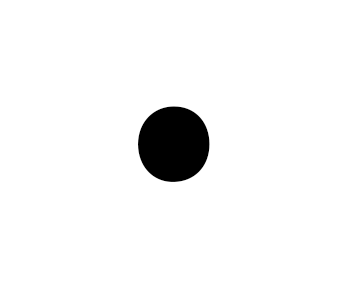
\includegraphics{fig1.png}}
\caption{Example of a figure caption.}
\label{fig}
\end{figure}

Figure Labels: Use 8 point Times New Roman for Figure labels. Use words 
rather than symbols or abbreviations when writing Figure axis labels to 
avoid confusing the reader. As an example, write the quantity 
``Magnetization'', or ``Magnetization, M'', not just ``M''. If including 
units in the label, present them within parentheses. Do not label axes only 
with units. In the example, write ``Magnetization (A/m)'' or ``Magnetization 
\{A[m(1)]\}'', not just ``A/m''. Do not label axes with a ratio of 
quantities and units. For example, write ``Temperature (K)'', not 
``Temperature/K''.

\section*{Acknowledgment}

The preferred spelling of the word ``acknowledgment'' in America is without 
an ``e'' after the ``g''. Avoid the stilted expression ``one of us (R. B. 
G.) thanks $\ldots$''. Instead, try ``R. B. G. thanks$\ldots$''. Put sponsor 
acknowledgments in the unnumbered footnote on the first page.

\section*{References}

Please number citations consecutively within brackets \cite{b1}. The 
sentence punctuation follows the bracket \cite{b2}. Refer simply to the reference 
number, as in \cite{b3}---do not use ``Ref. \cite{b3}'' or ``reference \cite{b3}'' except at 
the beginning of a sentence: ``Reference \cite{b3} was the first $\ldots$''

Number footnotes separately in superscripts. Place the actual footnote at 
the bottom of the column in which it was cited. Do not put footnotes in the 
abstract or reference list. Use letters for table footnotes.

Unless there are six authors or more give all authors' names; do not use 
``et al.''. Papers that have not been published, even if they have been 
submitted for publication, should be cited as ``unpublished'' \cite{b4}. Papers 
that have been accepted for publication should be cited as ``in press'' \cite{b5}. 
Capitalize only the first word in a paper title, except for proper nouns and 
element symbols.

For papers published in translation journals, please give the English 
citation first, followed by the original foreign-language citation \cite{b6}.

\begin{thebibliography}{00}
\bibitem{b1} Hadipour, Mojtaba and Hosseinzadeh, Ali and Sadidi, Mohsen. (2021). Investigation of the Stability of the Ball and Beam by the PID Controller. Journal of Manufacturing Technology Management. 51-58.
\bibitem{b2} Núñez, Acosta and Jiménez: Control of a ball-and-plate system using a State-feedback controller
\bibitem{b3}  Khalid Lefrouni, Younes Moubachir and Saoudi Taibi “Control of Ball-Plate System with Observer-Based State-Feedback and Geometric Considerations” International Journal of Difference Equations (IJDE). ISSN 0973-6069 Volume 16, Number 1 (2021), pp. 35-46
\bibitem{b4}Ali, H.I., Jassim, H.M. and Hasan, A.F. Optimal Nonlinear Model Reference Controller Design for Ball and Plate System. Arab J Sci Eng 44, 6757–6768 (2019)
\bibitem{b5} D. Meiling, L. Bingyou, L. Wang, “Position control for ball and beam system based on active disturbance rejection control”, Systems Science and Control Engineering. 7. 97-108. 10.1080/21642583.2019.1575297, 2019.
\bibitem{b6} Tudić, V., Kralj, D., Hoster, J., and Tropčić, T. (2022). Design and Implementation of a Ball-Plate Control System and Python Script for Educational Purposes in STEM Technologies. Sensors (Basel, Switzerland), 22(5), 1875. 
\bibitem{b7} A. Mujadin and A. A. Pratama, “High precession resistive touch screen driver circuitry for ball on plate balancing systems,” 2017 International Symposium on Electronics and Smart Devices (ISESD), Yogyakarta, 2017, pp. 242-246 
\bibitem{b8} Chi-Cheng Cheng and Chen-Hsun Tsai, “Visual Servo Control for Balancing a Ball-Plate System,” International Journal of Mechanical Engineering and Robotics Research, Vol. 5, No. 1, pp. 28-32, January 2016
\bibitem{b9} F. Dusek, D. Honc, and K. R. Sharma, “Modelling of ball and plate system based on first principal model and optimal control,” 2017 21st International Conference on Process Control (PC), Strbske Pleso, 2017, pp. 216-221
\bibitem{b10} I. M. Mehedi, U. M. Al-Saggaf, R. Mansouri, and M. Bettayeb, “Two degrees of freedom fractional controller design: Application to the ball and beam system,” Meas. J. Int. Meas. Confed., vol. 135, pp. 13–22, 2019, doi: 10.1016/j.measurement.2018.11.021. 
\bibitem{b11} Mohamed R. Elshamy, Essam Nabil1, Amged Sayed1 and Belal Abozalam1 “Enhancement of the Ball Balancing on the Plate using hybrid PD/Machine learning techniques” Journal of Physics: Conference Series. 2128 012028(2021)
\bibitem{b12} Kuncan, M., Kaplan, K., Acar, F., Kundack, I. M., and Ertunc, H. M. (2019). Fuzzy Logic Based Ball on Plate Balancing System Real Time Control by Image Processing. International Journal of Natural and Engineering Sciences, 10(3), 28–32.
\bibitem{b13} Alexander Hasp Frank, Morgan TJernstom “Construction and theoretical study of a ball balancing platform”KTH Royal Institue Of Technolgy School Of Industrial Engineering And Management(2019)
\bibitem{b14} Bang, Heeseung and Lee, Young. (2018). Implementation of a Ball and Plate Control System Using Sliding Mode Control. IEEE Access. PP. 1-1. 10.1109/ACCESS.2018.2838544.
\bibitem{b15}  Ernesto Fabregas, Sebastian Dormido-Canto, Sebasti ´ an´ Dormido, Virtual and Remote Laboratory with the Ball and Plate System, IFAC-PapersOnLine, Volume 50, Issue 1, 2017, Pages 9132-9137, ISSN 2405-8963
\end{thebibliography}
\vspace{12pt}
\color{red}
IEEE conference templates contain guidance text for composing and formatting conference papers. Please ensure that all template text is removed from your conference paper prior to submission to the conference. Failure to remove the template text from your paper may result in your paper not being published.

\end{document}